\documentclass{article}%
\usepackage[T1]{fontenc}%
\usepackage[utf8]{inputenc}%
\usepackage{lmodern}%
\usepackage{textcomp}%
\usepackage{lastpage}%
\usepackage{geometry}%
\geometry{tmargin=2cm,lmargin=2cm,rmargin=2cm,bmargin=2cm}%
\usepackage{graphicx}%
\usepackage{float}%
\usepackage{booktabs}%
\usepackage{rotating}%
%
\title{Relatório de Análise de Performance dos Modelos de Resposta}%
\date{\today}%
%
\begin{document}%
\normalsize%
\maketitle%
\section*{Introdução}%
\label{sec:Introduo}%
Este relatório apresenta uma análise completa dos modelos de resposta, avaliando a similaridade entre as respostas geradas e as respostas de referência. Foram calculadas diversas métricas de similaridade e realizadas análises estatísticas e visuais para identificar padrões de performance, inconsistências e possíveis pontos de melhoria. O objetivo é fornecer subsídios para interpretar os dados de forma objetiva, auxiliando na tomada de decisões para ajustes nos algoritmos.

%
\section*{Metodologia}%
\label{sec:Metodologia}%
A análise foi realizada em duas etapas principais:\newline%
\newline%
%
\begin{itemize}%
\item Carregamento dos dados: os dados foram extraídos de um arquivo pickle e convertidos para dicionários, possibilitando o acesso às respostas dos modelos e às respostas de referência.%
\item Processamento e análise: foram calculadas diversas métricas de similaridade, estatísticas descritivas e correlações. Além disso, foram gerados diversos gráficos (barras, histogramas, boxplots, heatmaps e scatter plots) para facilitar a interpretação visual dos resultados.%
\end{itemize}%
Cada gráfico ou tabela vem acompanhado de uma breve explicação sobre como interpretá{-}lo, de modo que o leitor possa compreender os pontos principais de cada análise.

%
\section*{Resultados}%
\label{sec:Resultados}%
\subsection*{Estatísticas de Similaridade Geral}%
\label{subsec:EstatsticasdeSimilaridadeGeral}%
Nesta seção são apresentadas as estatísticas descritivas da overall similarity dos modelos. Valores médios e medianos mais elevados indicam melhor aderência às respostas de referência, enquanto um alto desvio padrão pode indicar maior variabilidade.%
\newline%
Foram gerados os seguintes gráficos para visualizar esses dados:%


\begin{figure}[H]%
\centering%
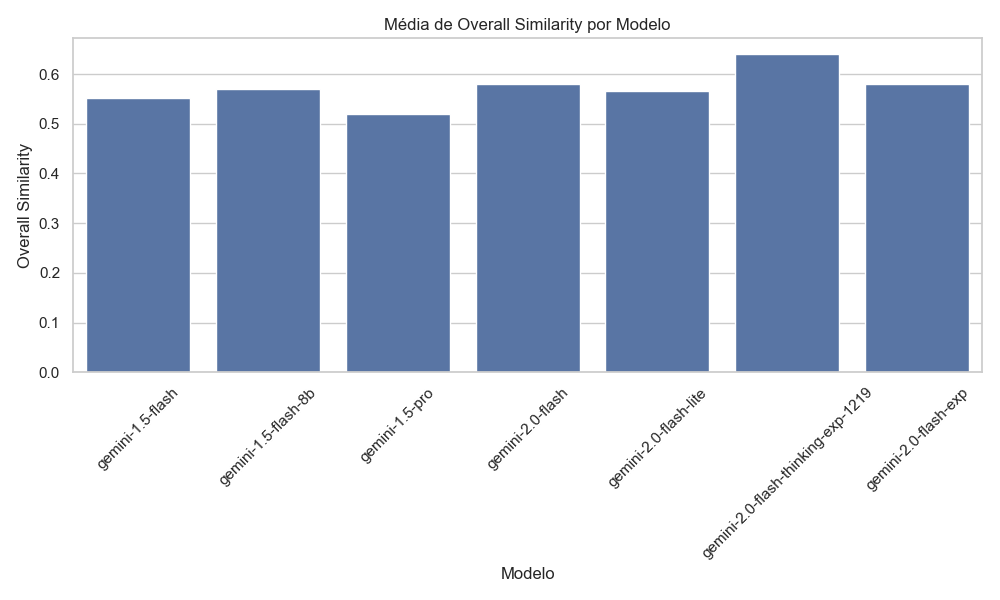
\includegraphics[width=0.8\textwidth]{analysis_results/barplot_overall_similarity.png}%
\caption{Gráfico de Barras – Média de Overall Similarity por Modelo. Observe as diferenças de desempenho entre os modelos.}%
\end{figure}

%


\begin{figure}[H]%
\centering%
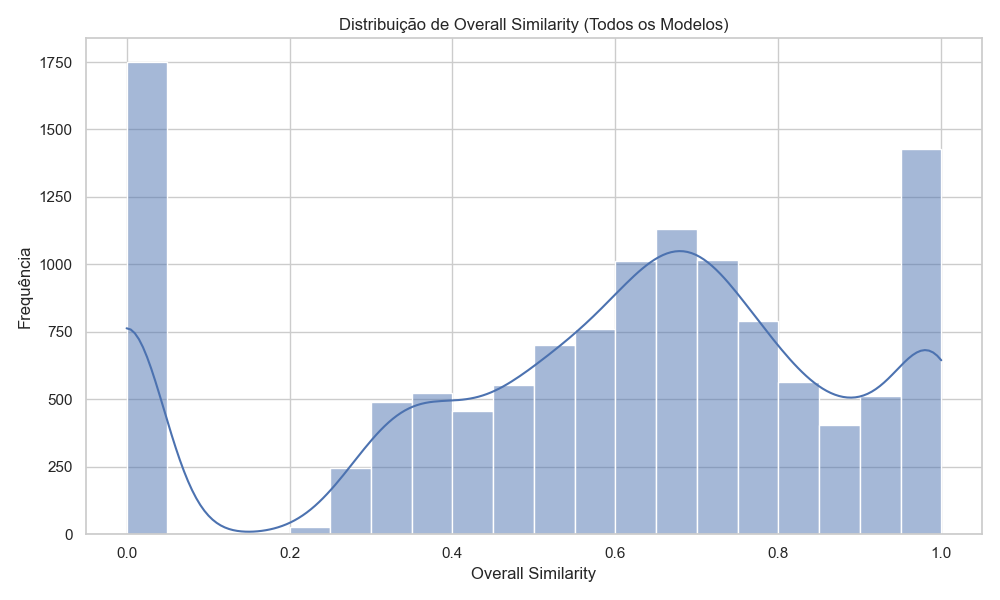
\includegraphics[width=0.8\textwidth]{analysis_results/histogram_overall_similarity.png}%
\caption{Histograma – Distribuição de Overall Similarity. Permite visualizar a dispersão dos valores obtidos.}%
\end{figure}

%


\begin{figure}[H]%
\centering%
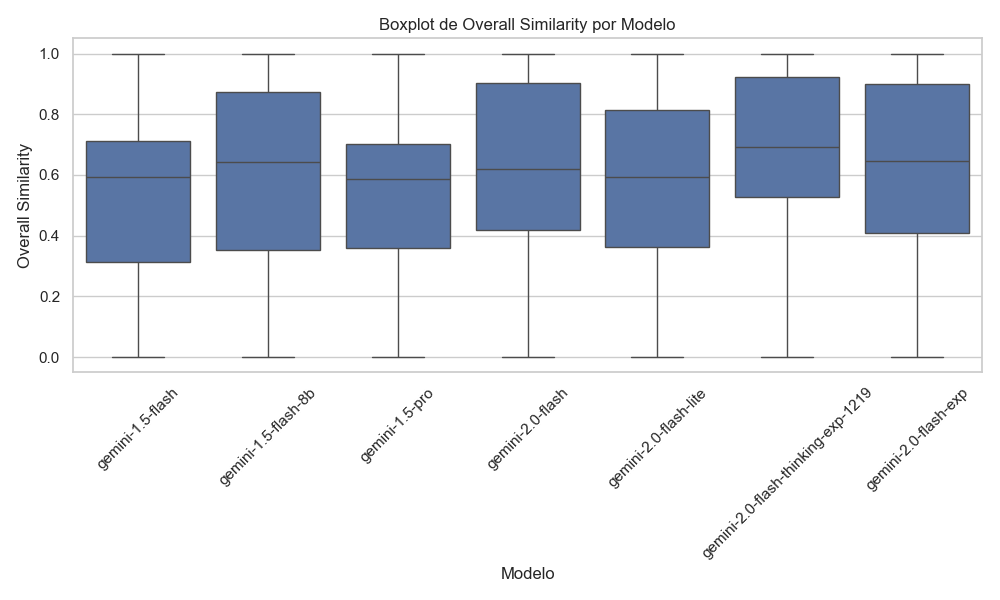
\includegraphics[width=0.8\textwidth]{analysis_results/boxplot_overall_similarity.png}%
\caption{Boxplot – Overall Similarity por Modelo. Facilita a identificação de mediana, quartis e outliers.}%
\end{figure}

%
\subsection*{Correlação entre Métricas de Similaridade}%
\label{subsec:CorrelaoentreMtricasdeSimilaridade}%
Nesta análise, avaliamos a correlação entre as diferentes métricas de similaridade (score keys). O heatmap abaixo mostra a força da correlação entre cada par de métricas: valores próximos de 1 ou {-}1 indicam forte correlação, enquanto valores próximos de 0 sugerem correlação fraca ou inexistente.%


\begin{figure}[H]%
\centering%
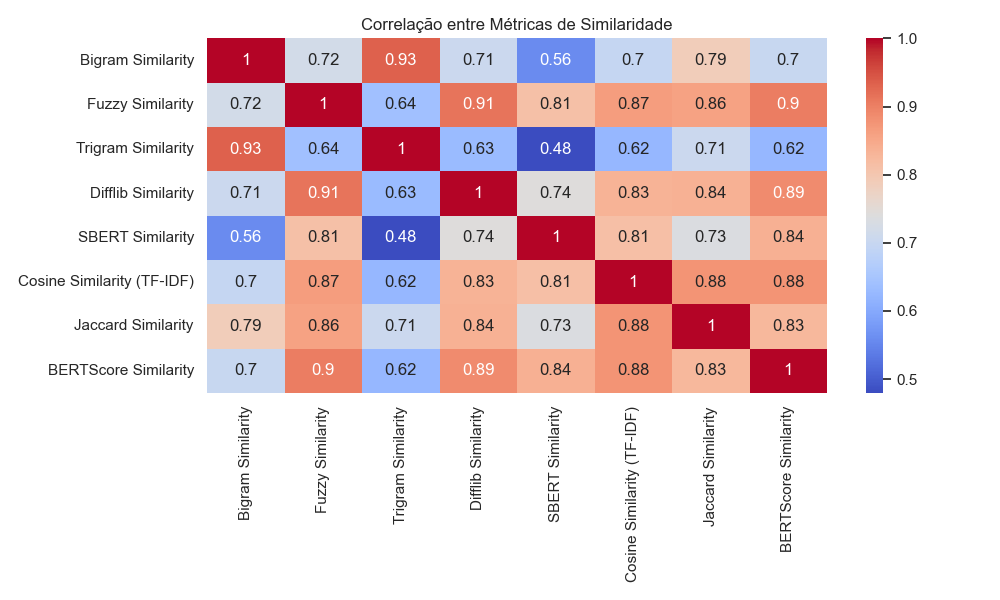
\includegraphics[width=0.8\textwidth]{analysis_results/heatmap_score_keys_correlation.png}%
\caption{Heatmap – Correlação entre as Métricas de Similaridade.}%
\end{figure}

%
\newline%
Além do heatmap, foram gerados scatter plots individuais comparando cada métrica com a overall similarity. Esses gráficos podem ser consultados nos anexos para análises mais detalhadas.

%
\subsection*{Correlação entre Overall Similarity e Média dos Scores}%
\label{subsec:CorrelaoentreOverallSimilarityeMdiadosScores}%
Esta seção apresenta a relação entre a overall similarity e a média dos scores detalhados (avg\textbackslash{}\_metric). O scatter plot a seguir permite identificar se existe uma tendência linear entre essas duas medidas, o que indicaria consistência na avaliação dos modelos.%


\begin{figure}[H]%
\centering%
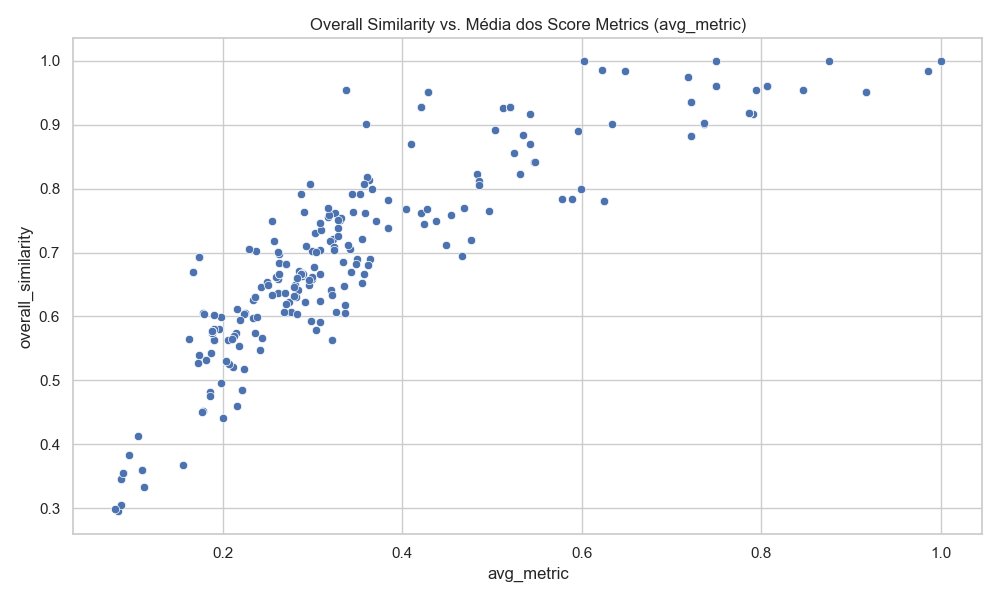
\includegraphics[width=0.8\textwidth]{analysis_results/scatter_overall_vs_avg_metric.png}%
\caption{Scatter Plot – Overall Similarity vs. Média dos Score Metrics (avg\textbackslash{}\_metric).}%
\end{figure}

%
\subsection*{Análise de Casos 'Unanswerable'}%
\label{subsec:AnlisedeCasosUnanswerable}%
Nesta parte, são analisados os casos em que os modelos não forneceram respostas (unanswerable). Os gráficos abaixo, apresentados lado a lado, mostram respectivamente a contagem desses casos e a relação entre a overall similarity e a condição de unanswerable. Em geral, uma baixa overall similarity pode estar associada a questões sem resposta.%


\begin{figure}[H]%
\begin{minipage}[b]{0.45\textwidth}%
\centering%
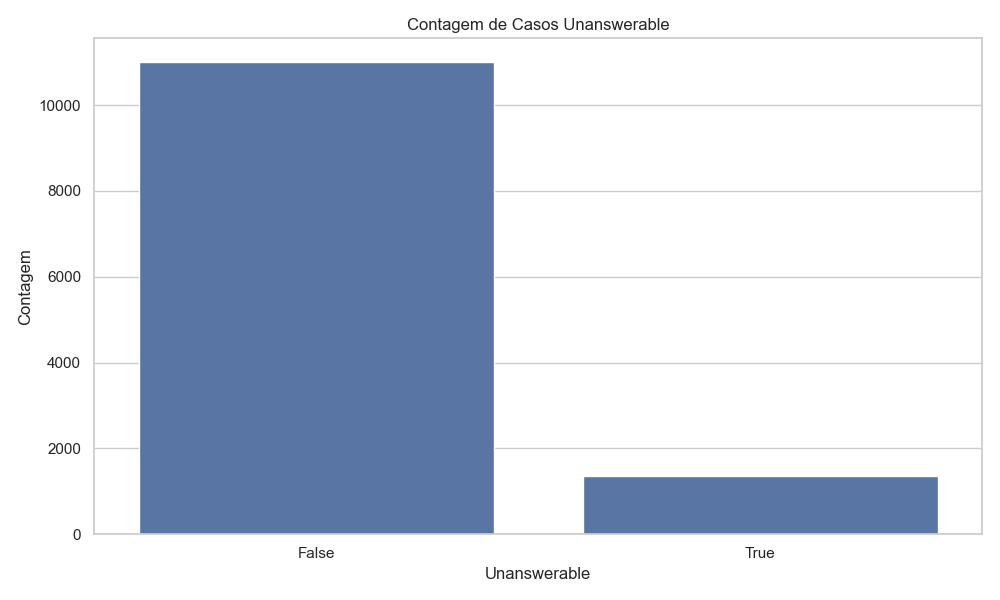
\includegraphics[width=\linewidth]{analysis_results/count_unanswerable.png}%
\caption*{Contagem de Casos Unanswerable.}%
\end{minipage}\hfill%
\begin{minipage}[b]{0.45\textwidth}%
\centering%
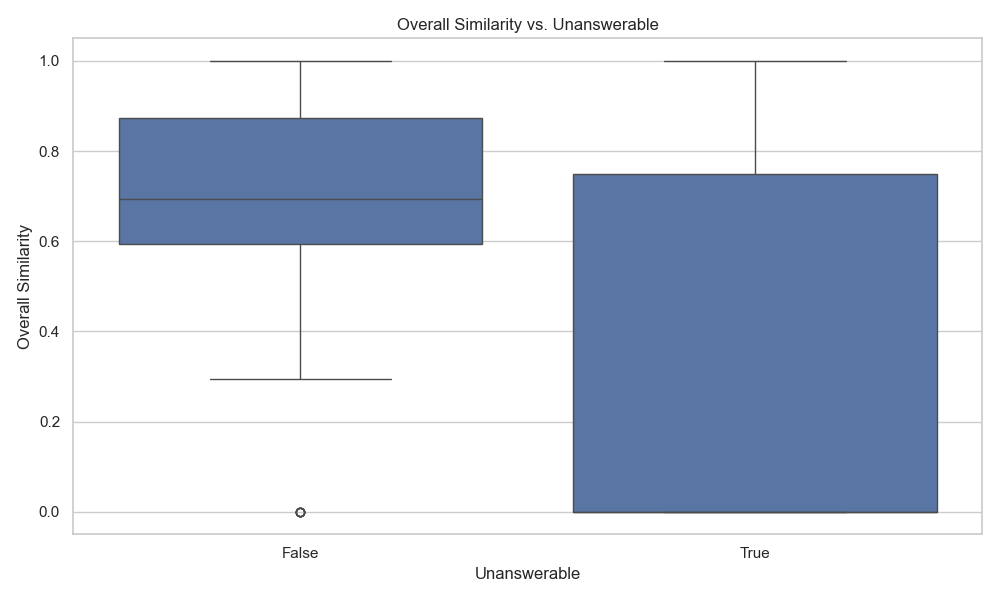
\includegraphics[width=\linewidth]{analysis_results/boxplot_overall_vs_unanswerable.png}%
\caption*{Boxplot – Overall Similarity vs. Unanswerable.}%
\end{minipage}%
\end{figure}

%
\subsection*{Correlação Inter{-}Modelos}%
\label{subsec:CorrelaoInter{-}Modelos}%
Esta análise verifica a correlação da overall similarity entre os diferentes modelos. Utilizando uma pivot table, foi calculada a correlação entre os modelos, cuja visualização por meio de um heatmap facilita a identificação de similaridades ou discrepâncias na performance entre eles.%


\begin{figure}[H]%
\centering%
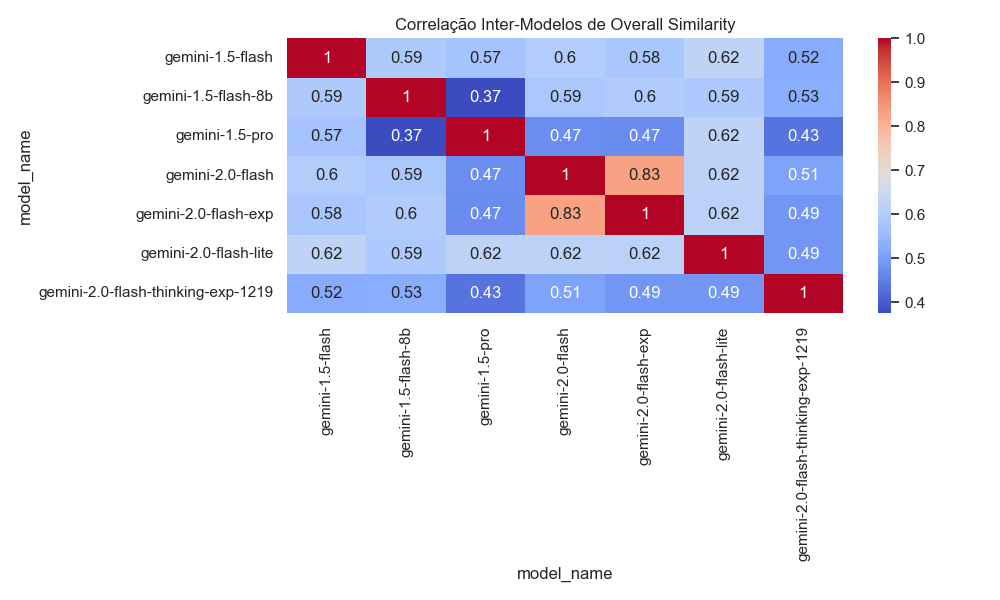
\includegraphics[width=0.8\textwidth]{analysis_results/heatmap_inter_model_corr.png}%
\caption{Heatmap – Correlação Inter{-}Modelos de Overall Similarity.}%
\end{figure}

%
\subsection*{Estatísticas Agregadas das Métricas Detalhadas}%
\label{subsec:EstatsticasAgregadasdasMtricasDetalhadas}%
A seguir, serão apresentadas diversas tabelas, cada uma correspondendo a um score específico. Em cada tabela, estão exibidas as estatísticas agregadas – média, mediana, desvio padrão, valor mínimo e valor máximo – agrupadas por modelo. Essas métricas auxiliam na identificação de padrões e na avaliação da consistência dos scores obtidos.%
\subsubsection*{Estatísticas para o Score: aggregated\_BERTScore Similarity}%
\begin{table}[H]%
\centering%
\begin{tabular}{llllll}
\toprule
 & mean & median & std & min & max \\
model_name &  &  &  &  &  \\
\midrule
gemini-1.5-flash & 0.6915 & 0.6883 & 0.1026 & 0.5161 & 1.0000 \\
gemini-1.5-flash-8b & 0.7623 & 0.7315 & 0.1252 & 0.5615 & 1.0000 \\
gemini-1.5-pro & 0.6677 & 0.6666 & 0.0812 & 0.5169 & 0.8922 \\
gemini-2.0-flash & 0.7546 & 0.7383 & 0.1239 & 0.5616 & 1.0000 \\
gemini-2.0-flash-exp & 0.7573 & 0.7462 & 0.1245 & 0.5544 & 1.0000 \\
gemini-2.0-flash-lite & 0.7327 & 0.7033 & 0.1269 & 0.5263 & 1.0000 \\
gemini-2.0-flash-thinking-exp-1219 & 0.7734 & 0.7575 & 0.1259 & 0.5263 & 1.0000 \\
\bottomrule
\end{tabular}
%
\end{table}%
\vspace{0.5cm}%
\subsubsection*{Estatísticas para o Score: aggregated\_Bigram Similarity}%
\begin{table}[H]%
\centering%
\begin{tabular}{llllll}
\toprule
 & mean & median & std & min & max \\
model_name &  &  &  &  &  \\
\midrule
gemini-1.5-flash & 0.0620 & 0.0167 & 0.1370 & 0.0000 & 1.0000 \\
gemini-1.5-flash-8b & 0.1296 & 0.0000 & 0.2651 & 0.0000 & 1.0000 \\
gemini-1.5-pro & 0.0475 & 0.0098 & 0.1039 & 0.0000 & 1.0000 \\
gemini-2.0-flash & 0.1416 & 0.0000 & 0.2597 & 0.0000 & 1.0000 \\
gemini-2.0-flash-exp & 0.1468 & 0.0000 & 0.2585 & 0.0000 & 1.0000 \\
gemini-2.0-flash-lite & 0.1227 & 0.0000 & 0.2472 & 0.0000 & 1.0000 \\
gemini-2.0-flash-thinking-exp-1219 & 0.1151 & 0.0000 & 0.2453 & 0.0000 & 1.0000 \\
\bottomrule
\end{tabular}
%
\end{table}%
\vspace{0.5cm}%
\subsubsection*{Estatísticas para o Score: aggregated\_Cosine Similarity (TF-IDF)}%
\begin{table}[H]%
\centering%
\begin{tabular}{llllll}
\toprule
 & mean & median & std & min & max \\
model_name &  &  &  &  &  \\
\midrule
gemini-1.5-flash & 0.2878 & 0.2451 & 0.2381 & 0.0000 & 1.0000 \\
gemini-1.5-flash-8b & 0.4042 & 0.3306 & 0.3446 & 0.0000 & 1.0000 \\
gemini-1.5-pro & 0.2385 & 0.2088 & 0.1784 & 0.0000 & 1.0000 \\
gemini-2.0-flash & 0.4074 & 0.3161 & 0.3337 & 0.0000 & 1.0000 \\
gemini-2.0-flash-exp & 0.4161 & 0.3510 & 0.3321 & 0.0000 & 1.0000 \\
gemini-2.0-flash-lite & 0.3612 & 0.2688 & 0.3306 & 0.0000 & 1.0000 \\
gemini-2.0-flash-thinking-exp-1219 & 0.4525 & 0.3800 & 0.3657 & 0.0000 & 1.0000 \\
\bottomrule
\end{tabular}
%
\end{table}%
\vspace{0.5cm}%
\subsubsection*{Estatísticas para o Score: aggregated\_Difflib Similarity}%
\begin{table}[H]%
\centering%
\begin{tabular}{llllll}
\toprule
 & mean & median & std & min & max \\
model_name &  &  &  &  &  \\
\midrule
gemini-1.5-flash & 0.2217 & 0.1626 & 0.2347 & 0.0000 & 1.0000 \\
gemini-1.5-flash-8b & 0.3814 & 0.2693 & 0.3356 & 0.0000 & 1.0000 \\
gemini-1.5-pro & 0.1752 & 0.1389 & 0.1664 & 0.0035 & 0.9855 \\
gemini-2.0-flash & 0.4000 & 0.3210 & 0.3142 & 0.0000 & 1.0000 \\
gemini-2.0-flash-exp & 0.4105 & 0.3293 & 0.3168 & 0.0000 & 1.0000 \\
gemini-2.0-flash-lite & 0.3557 & 0.2561 & 0.3145 & 0.0000 & 1.0000 \\
gemini-2.0-flash-thinking-exp-1219 & 0.4142 & 0.3429 & 0.3276 & 0.0000 & 1.0000 \\
\bottomrule
\end{tabular}
%
\end{table}%
\vspace{0.5cm}%
\subsubsection*{Estatísticas para o Score: aggregated\_Fuzzy Similarity}%
\begin{table}[H]%
\centering%
\begin{tabular}{llllll}
\toprule
 & mean & median & std & min & max \\
model_name &  &  &  &  &  \\
\midrule
gemini-1.5-flash & 0.2808 & 0.2550 & 0.2353 & 0.0000 & 1.0000 \\
gemini-1.5-flash-8b & 0.4393 & 0.3800 & 0.3101 & 0.0000 & 1.0000 \\
gemini-1.5-pro & 0.2368 & 0.2150 & 0.1773 & 0.0100 & 0.9900 \\
gemini-2.0-flash & 0.4731 & 0.4050 & 0.2784 & 0.0000 & 1.0000 \\
gemini-2.0-flash-exp & 0.4736 & 0.4100 & 0.2838 & 0.0000 & 1.0000 \\
gemini-2.0-flash-lite & 0.4147 & 0.3800 & 0.2906 & 0.0000 & 1.0000 \\
gemini-2.0-flash-thinking-exp-1219 & 0.4672 & 0.4300 & 0.3022 & 0.0000 & 1.0000 \\
\bottomrule
\end{tabular}
%
\end{table}%
\vspace{0.5cm}%
\subsubsection*{Estatísticas para o Score: aggregated\_Jaccard Similarity}%
\begin{table}[H]%
\centering%
\begin{tabular}{llllll}
\toprule
 & mean & median & std & min & max \\
model_name &  &  &  &  &  \\
\midrule
gemini-1.5-flash & 0.1584 & 0.1181 & 0.1973 & 0.0000 & 1.0000 \\
gemini-1.5-flash-8b & 0.2925 & 0.1572 & 0.3416 & 0.0000 & 1.0000 \\
gemini-1.5-pro & 0.1224 & 0.0947 & 0.1291 & 0.0000 & 1.0000 \\
gemini-2.0-flash & 0.2897 & 0.1557 & 0.3173 & 0.0000 & 1.0000 \\
gemini-2.0-flash-exp & 0.3005 & 0.1667 & 0.3140 & 0.0000 & 1.0000 \\
gemini-2.0-flash-lite & 0.2477 & 0.1429 & 0.2971 & 0.0000 & 1.0000 \\
gemini-2.0-flash-thinking-exp-1219 & 0.3201 & 0.1731 & 0.3563 & 0.0000 & 1.0000 \\
\bottomrule
\end{tabular}
%
\end{table}%
\vspace{0.5cm}%
\subsubsection*{Estatísticas para o Score: aggregated\_SBERT Similarity}%
\begin{table}[H]%
\centering%
\begin{tabular}{llllll}
\toprule
 & mean & median & std & min & max \\
model_name &  &  &  &  &  \\
\midrule
gemini-1.5-flash & 0.5236 & 0.5631 & 0.2719 & -0.0514 & 1.0000 \\
gemini-1.5-flash-8b & 0.6359 & 0.6527 & 0.2842 & -0.0237 & 1.0000 \\
gemini-1.5-pro & 0.4936 & 0.5351 & 0.2436 & -0.0602 & 0.9894 \\
gemini-2.0-flash & 0.6146 & 0.6067 & 0.2808 & -0.0191 & 1.0000 \\
gemini-2.0-flash-exp & 0.6195 & 0.6277 & 0.2811 & -0.0191 & 1.0000 \\
gemini-2.0-flash-lite & 0.5457 & 0.5590 & 0.3069 & -0.0884 & 1.0000 \\
gemini-2.0-flash-thinking-exp-1219 & 0.6779 & 0.6746 & 0.2653 & 0.0374 & 1.0000 \\
\bottomrule
\end{tabular}
%
\end{table}%
\vspace{0.5cm}%
\subsubsection*{Estatísticas para o Score: aggregated\_Trigram Similarity}%
\begin{table}[H]%
\centering%
\begin{tabular}{llllll}
\toprule
 & mean & median & std & min & max \\
model_name &  &  &  &  &  \\
\midrule
gemini-1.5-flash & 0.0387 & 0.0000 & 0.1281 & 0.0000 & 1.0000 \\
gemini-1.5-flash-8b & 0.1052 & 0.0000 & 0.2567 & 0.0000 & 1.0000 \\
gemini-1.5-pro & 0.0284 & 0.0000 & 0.0961 & 0.0000 & 1.0000 \\
gemini-2.0-flash & 0.1136 & 0.0000 & 0.2457 & 0.0000 & 1.0000 \\
gemini-2.0-flash-exp & 0.1161 & 0.0000 & 0.2445 & 0.0000 & 1.0000 \\
gemini-2.0-flash-lite & 0.1039 & 0.0000 & 0.2389 & 0.0000 & 1.0000 \\
gemini-2.0-flash-thinking-exp-1219 & 0.0839 & 0.0000 & 0.2209 & 0.0000 & 1.0000 \\
\bottomrule
\end{tabular}
%
\end{table}%
\vspace{0.5cm}

%
\section*{Discussão}%
\label{sec:Discusso}%

A análise dos dados indica que o modelo \textbf{gemini-2.0-flash-thinking-exp-1219} apresentou a maior média de overall similarity (0.65), 
enquanto o modelo \textbf{gemini-1.5-flash} apresentou a menor média (0.50). Essa diferença ressalta variações na performance 
dos modelos em aderência às respostas de referência.

Adicionalmente, observa-se que o percentual de casos com dicionário de scores vazio foi mais elevado para o modelo 
\textbf{gemini-1.5-flash-8b} (25.0%), sugerindo que podem haver dificuldades na geração ou na coleta dos scores para esse modelo.

A análise das estatísticas agregadas das métricas detalhadas evidencia variações na consistência dos modelos, o que pode ser explorado 
para identificar possíveis ajustes nos algoritmos de resposta.

%
\section*{Conclusões}%
\label{sec:Concluses}%

Com base nos dados analisados, pode-se concluir que:
\begin{itemize}
    \item Modelos com maiores médias de overall similarity tendem a aderir melhor às respostas de referência, embora a variabilidade dos scores deva ser considerada.
    \item O elevado percentual de casos com scores vazios em alguns modelos indica a necessidade de investigar a qualidade dos dados e o processo de geração de scores.
    \item As estatísticas agregadas das métricas detalhadas oferecem insights sobre a consistência dos modelos, o que pode orientar ajustes para aprimorar a performance.
\end{itemize}

%
\section*{Anexos}%
\label{sec:Anexos}%
Os anexos deste relatório reúnem os arquivos CSV gerados e todos os gráficos produzidos durante a análise, tais como:%
\begin{itemize}%
\item overall\_stats.csv%
\item empty\_scores\_frequency.csv%
\item variation\_data.csv%
\item aggregated\_metrics.csv%
\item overall\_similarity.csv%
\item detailed\_similarity.csv%
\end{itemize}%
Além disso, todos os gráficos (barplots, histogramas, boxplots, heatmaps e scatter plots) podem ser conferidos na pasta 'analysis\_results'.

%
\section*{Referências}%
\label{sec:Referncias}%
As principais bibliotecas e ferramentas utilizadas para a geração deste relatório foram:%
\begin{itemize}%
\item \textbf{pandas} e \textbf{numpy} para manipulação e análise dos dados.%
\item \textbf{matplotlib} e \textbf{seaborn} para a criação dos gráficos.%
\item \textbf{PyLaTeX} para a montagem do documento LaTeX.%
\end{itemize}

%
\end{document}